\documentclass{beamer}
 
\usepackage[utf8]{inputenc}
 
\usetheme{Madrid} 

\usepackage{natbib}
\bibliographystyle{chicago}

\begin{document}

\title[Math 4P06 Presentation] %optional
{Estimating time-varying transmission rates in the SIR model}

\author[Sang Woo Park] % (optional, for multiple authors)
{Sang Woo Park}

\institute[McMaster University] % (optional)
{
    Department of Mathematics and Statistics\\
    McMaster University
}

\date[2019] % (optional)
{April 10, 2019}

\frame{\titlepage}

\begin{frame}
\frametitle{Epidemic time series}
\begin{itemize}
    \item Measles report (prior to vaccination)
\end{itemize}
\begin{center}
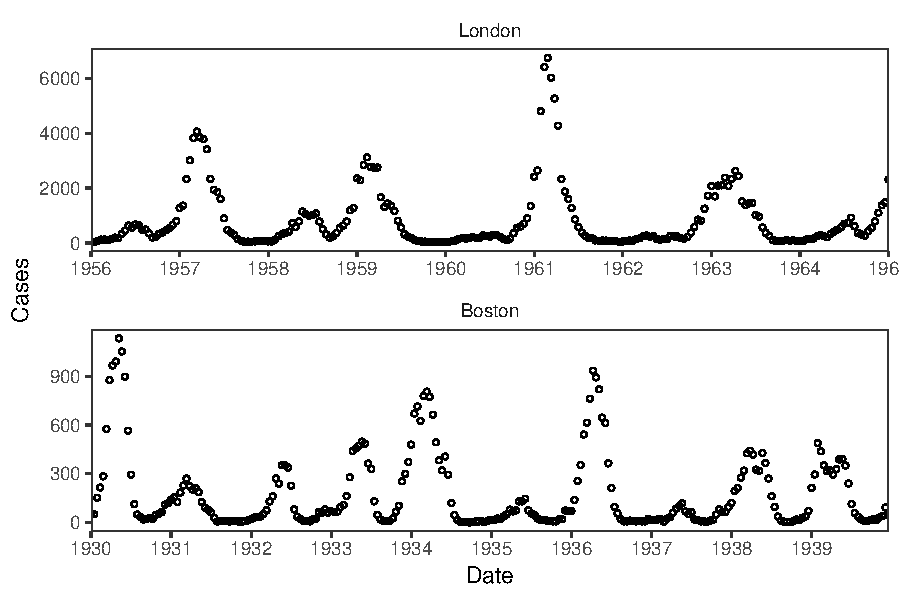
\includegraphics[width=0.9\textwidth]{fig1.pdf}
\end{center}
\end{frame}

\begin{frame}
\frametitle{Susceptible-Infected-Recovered (SIR) model}
\begin{itemize}
    \item Describes how disease spreads in a population \citep{kermack1927contribution}
\end{itemize}
\begin{center}
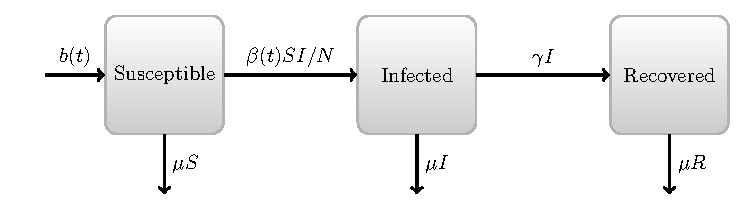
\includegraphics[width=\textwidth]{model_diagram.pdf}
\end{center}
\end{frame}

\begin{frame}
\frametitle{Susceptible-Infected-Recovered (SIR) model}
$$
\begin{aligned}
\frac{dS}{dt} &= b(t) - \beta(t) S \frac{I}{N} - \mu S\\
\frac{dI}{dt} &= \beta(t) S \frac{I}{N} - (\gamma + \mu) I\\
\frac{dR}{dt} &= \gamma I - \mu R
\end{aligned}
$$
\begin{itemize}
	\item Mean infectious period $1/\gamma$
	\item Mean life expectancy $1/\mu$
	\item Birth rate $b(t)$
	\item Contact rate $\beta(t)$
\end{itemize}
\end{frame}

\begin{frame}
\frametitle{Trajectory matching}
\begin{itemize}
	\item Try to match the solution of the ODE with the observed time series
\end{itemize}
\begin{center}
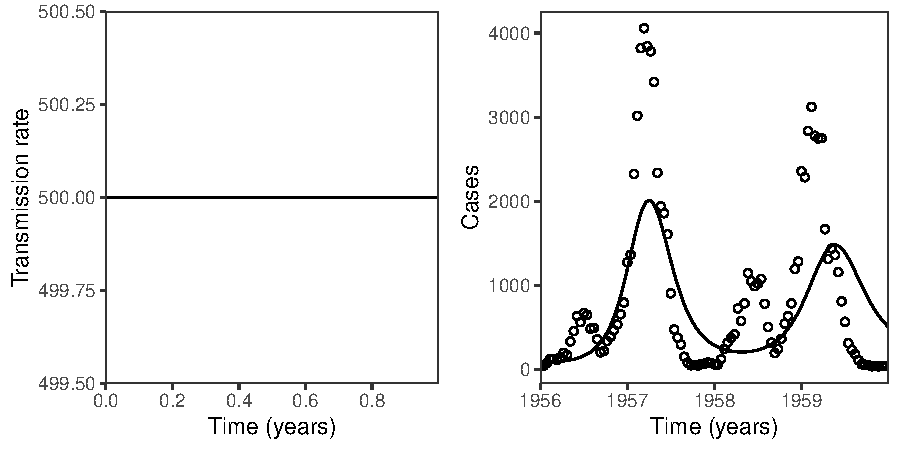
\includegraphics[width=\textwidth]{traj1.pdf}
\end{center}
\end{frame}

\begin{frame}
\frametitle{Trajectory matching}
\begin{itemize}
	\item Try to match the solution of the ODE with the observed time series
\end{itemize}
\begin{center}
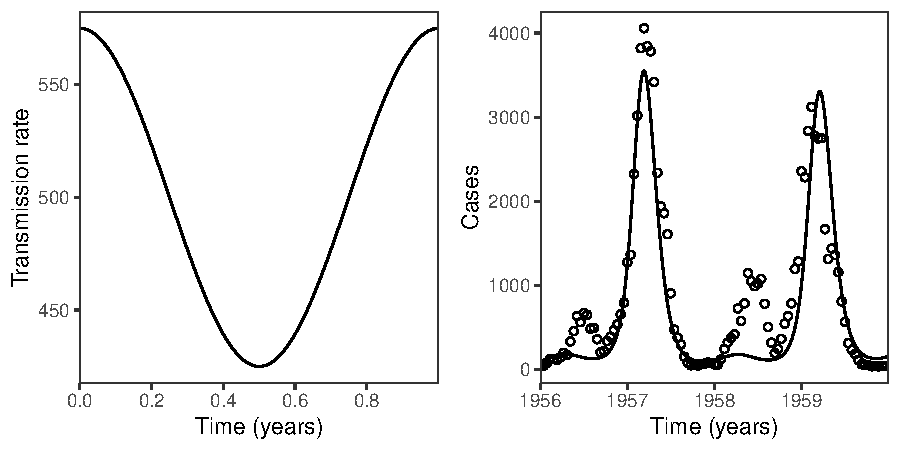
\includegraphics[width=\textwidth]{traj2.pdf}
\end{center}
\end{frame}

\begin{frame}
\frametitle{Trajectory matching}
\begin{itemize}
	\item Try to match the solution of the ODE with the observed time series
\end{itemize}
\begin{center}
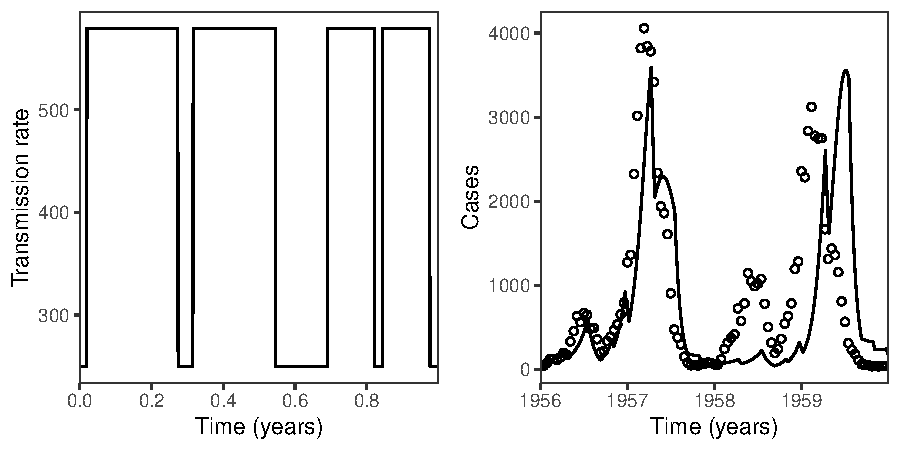
\includegraphics[width=\textwidth]{traj3.pdf}
\end{center}
\end{frame}

\begin{frame}
\frametitle{Sequential Monte Carlo (SMC)}
\begin{itemize}
	\item Probabilistic transition between states based on rate equations
	\item Use stochastic simulations to integrate over the state space \citep{king2015statistical}
\end{itemize}
\begin{center}
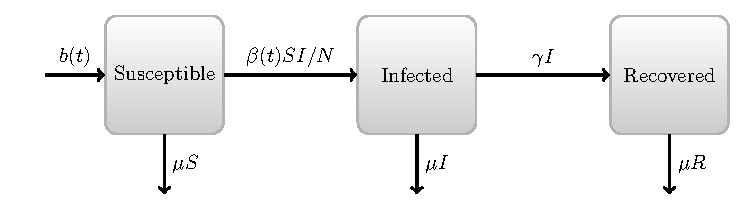
\includegraphics[width=\textwidth]{model_diagram.pdf}
\end{center}
\end{frame}

\begin{frame}
\frametitle{Non-exponential distributions}
\begin{itemize}
	\item SIR model assumes exponentially distributed generation time
	\item Realistic distributions are likely to be narrower \citep{simpson1952infectiousness, cori2013new}
\end{itemize}
\begin{center}
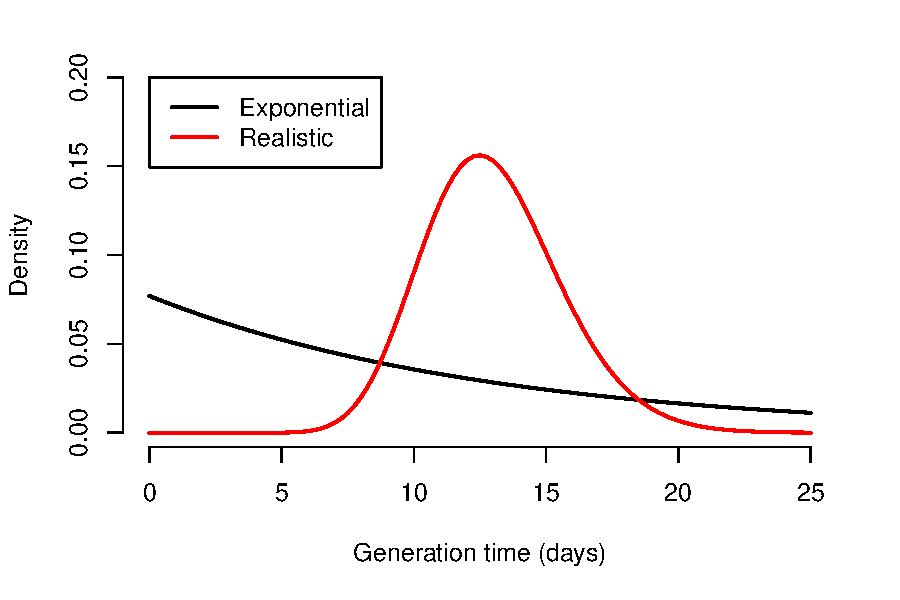
\includegraphics[width=0.8\textwidth]{distribution.pdf}
\end{center}
\end{frame}

\begin{frame}
\frametitle{The renewal equation}
\begin{itemize}
	\item Current incidence as a function of previous incidence and generation time distribution
	$$
	i(t) = \mathcal R(t) S(t) \int i(t-s) g(s) ds
	$$
	\begin{itemize}
	\itemsep0.7em
	\item Incidence $i(t)$
	\item Generation time distribution $g(t)$
	\item Scaled-transmission rate $\mathcal R(t) = \beta(t)/\gamma$
	\end{itemize}
\end{itemize}
\end{frame}

\begin{frame}
\frametitle{Time-series SIR model}
\begin{itemize}
	\item Begin by discretizing the system
	$$
	\begin{aligned}
	S_{t+1} &= B_t + S_t - i_{t+1}\\
	i_{t+1} &= \beta_t S_t \frac{i_t^\alpha}{N} 
	\end{aligned}
	$$
\end{itemize}
\end{frame}

\begin{frame}
\frametitle{Time-series SIR model}
\begin{itemize}
	\item Estimate the transmission rates using regression \citep{finkenstadt2000time}
	$$
	\log i_{t+1} = \log \beta_t + \log S_t + \alpha \log i_t - \log N + \epsilon_t
	$$
	\item Key assumptions:
	\begin{itemize}
		\item Fixed generation time
		\item No observation error (only process error)
		\item Power-law infection term
	\end{itemize}
\end{itemize}
\end{frame}

\begin{frame}
\frametitle{Relative bias}
\begin{itemize}
	\itemsep0.5em
	\item Relative bias: mean ratio between the estimates and the true value
	\item TSIR results in more than twofold bias
\end{itemize}
\begin{center}
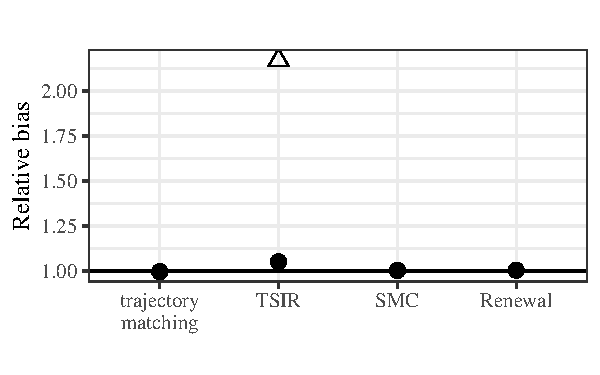
\includegraphics[width=0.8\textwidth]{bias.pdf}
\end{center}
\end{frame}

\begin{frame}
\frametitle{Coverage}
\begin{itemize}
	\item Coverage: proportion of confidence intervals that contain the true value
	\item Ignoring process error gives overconfident results \citep{king2015avoidable, taylor2016stochasticity}
	\item Ignoring observation error may give underconfident results
\end{itemize}
\begin{center}
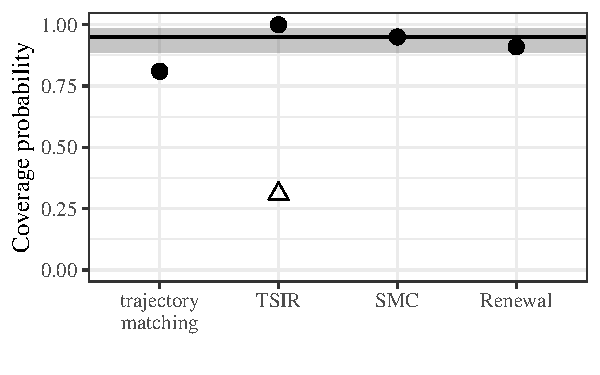
\includegraphics[width=0.8\textwidth]{coverage.pdf}
\end{center}
\end{frame}

\begin{frame}
\frametitle{Estimating time-varying transmission rates}
\begin{center}
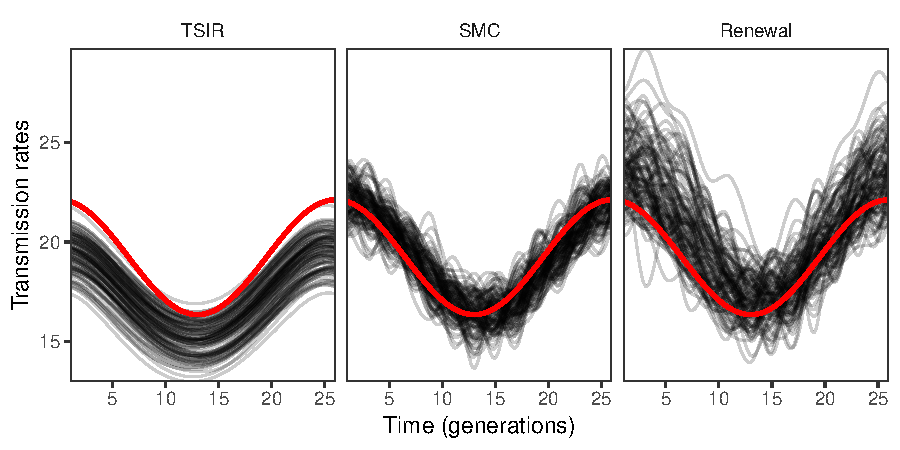
\includegraphics[width=\textwidth]{transmission.pdf}
\end{center}
\end{frame}

\begin{frame}
\frametitle{Generation-time distribution}
\begin{itemize}
	\item The shape of the generation-time distribution has little effect on overall dynamics
\end{itemize}
\begin{center}
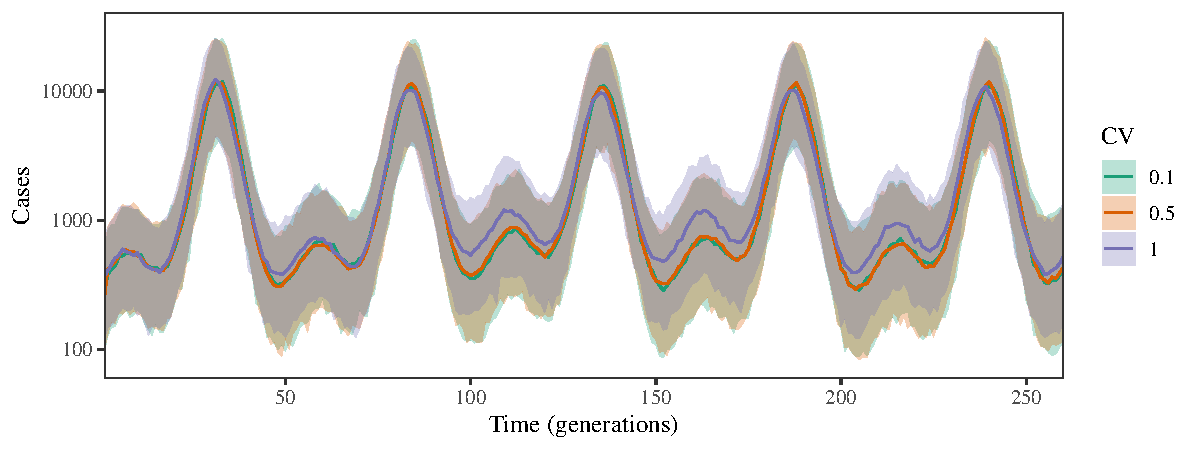
\includegraphics[width=\textwidth]{../figure/test_renewal_distribution.pdf}
\end{center}
\end{frame}

\begin{frame}
\frametitle{Amount of process and observation error}
\begin{itemize}
	\item Decompose residual variance from TSIR into process and observation variance
	\item Measles is largely driven by process error ($> 95\%$)
\end{itemize}
\begin{center}
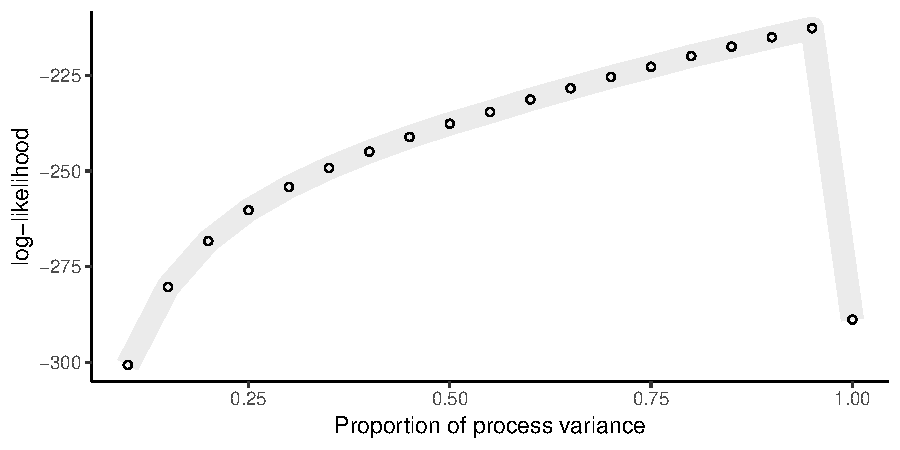
\includegraphics[width=\textwidth]{process.pdf}
\end{center}
\end{frame}

\begin{frame}
\frametitle{Probability of infection}
\begin{itemize}
	\item Power-law probability of infection, $\beta I^\alpha/N$, does not match the observed patterns 
	\item Small mismatch is expected when the probability of infection is small
\end{itemize}
\begin{center}
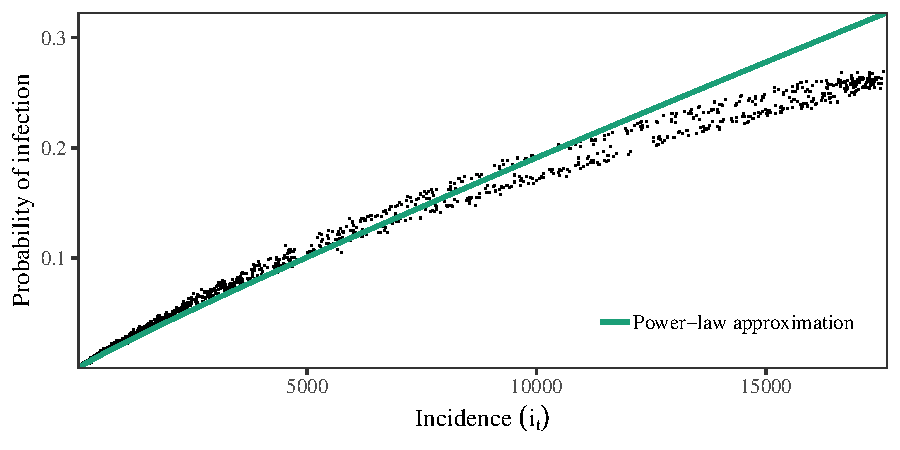
\includegraphics[width=0.8\textwidth]{poi.pdf}
\end{center}
\end{frame}

\begin{frame}
\frametitle{Conclusion}
\begin{itemize}
	\itemsep1em
	\item Regression-based methods:
	\begin{itemize}
		\item Fast and easy to implement
		\item Can estimate the exact shape of the transmission rates but give biased answers
		\item Good for exploratory analysis
	\end{itemize}
	\item Simulation-based methods:
	\begin{itemize}
		\item Computationally expensive
		\item Give unbiased answers with good coverage properties
		\item Hybrid approach? \citep{hooker2010parameterizing}
	\end{itemize}
	\item Using simulations can help us assess which assumptions are important
\end{itemize}
\end{frame}

\begin{frame}
\frametitle{References}
\tiny
\bibliography{thesis}
\end{frame}

\end{document}
